\section{Historical TON evidence and development record}
\subsection{Development evidence motivating the final comparison}
Development on C proceeded through four recorded stages. These stages answer different questions and are not a single ranking of competing algorithms. In the initial adaptation study, selecting updates using evidence of score inversion outperformed a random schedule with the same number of updates in mean block AUROC by 0.0217, 0.0559, and 0.0719 for logistic regression, an MLP, and the additive spline model, respectively, against the mean of 20 random schedules. For the additive spline model, none of these update policies exceeded the frozen mean block AUROC of 0.8911: evidence-driven, continuous, and random updates attained 0.8341, 0.8073, and 0.7621. The fitted-memory inversion diagnostic was in sample, and out-of-sample evidence from requested block labels was often unavailable or weak after the required delay. Improved ranking did not consistently improve both error counts.

The next stage changed the memory policy while retaining a 256-example capacity. For the continuously updated spline model, class-aware memory increased mean block AUROC by about 0.084 compared with global FIFO, while attack recall fell by 56.66 percentage points at the fixed historical threshold. Subsequent threshold experiments showed why score and decision changes had to be separated. Re-selecting only the frozen spline threshold improved recall on C by 17.73 percentage points and increased FPR by 1.48 percentage points, with exactly unchanged AUROC. Recalibration using the entire B archive was also explored during development, but that configuration required the additional historical archive and is not presented as satisfying the final 256-example online-memory contract.

The final development configuration separated FIT192 and ROLE64. For seed 42 on C, FIT192 / ROLE64 reduced FPR by 16.08 percentage points relative to Frozen / ROLE64, but reduced recall by 2.60 percentage points and mean block AUROC by about 0.109. This mixed outcome motivated preserving the four traces and reporting FN and FP separately in the final evaluation. The C findings are development evidence, not an additional independent confirmation of the final D result.

\subsection{Absolute outcomes on the final interval}
Tables~\ref{tab:rates} and~\ref{tab:counts} report all four traces, including the controls that retain the B threshold. With frozen weights, recent threshold selection raises mean attack recall on all D from $21.11\%$ to $89.09\%$, while FPR rises from $12.64\%$ to $46.74\%$. Mean block AUROC remains $0.8536$ because the scores are identical. Thus, a large recovery in recall can arise entirely from moving the decision threshold.

\begin{table}[tb]
\centering\fontsize{8.6}{10.5}\selectfont
\setlength{\tabcolsep}{4pt}
\caption{Final rates: mean $\pm$ sample SD over five paired seeds. Recall, FPR, and BA are percentages calculated globally. AUROC is the unweighted mean over valid blocks (352/355 for all D; 350/355 for A/B/C-unseen vectors), then averaged over seeds.}
\label{tab:rates}
\begin{tabular}{lrrrr}
\toprule
Trace & Recall (\%) & FPR (\%) & BA (\%) & Mean block AUROC \\
\midrule
\tablerows{tables/rates_rows.tex}
\bottomrule
\end{tabular}
\end{table}

\begin{table}[tb]
\centering\small
\caption{Absolute final error counts: mean $\pm$ sample SD over five seeds. Noninteger means result from averaging integer counts. The paired differences in Table~\ref{tab:paired} retain the seed correspondence.}
\label{tab:counts}
\begin{tabular}{lrr}
\toprule
Trace & False negatives & False positives \\
\midrule
\tablerows{tables/counts_rows.tex}
\bottomrule
\end{tabular}
\end{table}

The FIT192/B diagnostic displays the expected risk of retaining a threshold after changing the fitted sample and score scale. FIT192 / B reaches mean block AUROC $0.9359$, yet attack recall is only $8.81\%$ and FPR is $0.88\%$. The ranking improves on average, but the inherited threshold misses most attacks. Refitting with approximately balanced class quotas differs from fitting A, where about 94\% of observations are attacks. Under pure prior shift, the log-odds correction would be an intercept shift; here reweighted slopes and changing class-conditional traffic also contribute. Thus this control illustrates score--threshold mismatch rather than a newly discovered property of logistic models. With the same adapted scores and a recent threshold, FIT192 / ROLE64 reaches recall $89.38\%$ and FPR $20.47\%$. Relative to FIT192 / B, this threshold change removes 2,610,759.8 mean false negatives at the cost of 60,637.6 additional false positives. Figure~\ref{fig:operating} shows the resulting operating-point changes.

\begin{figure}[tb]
\centering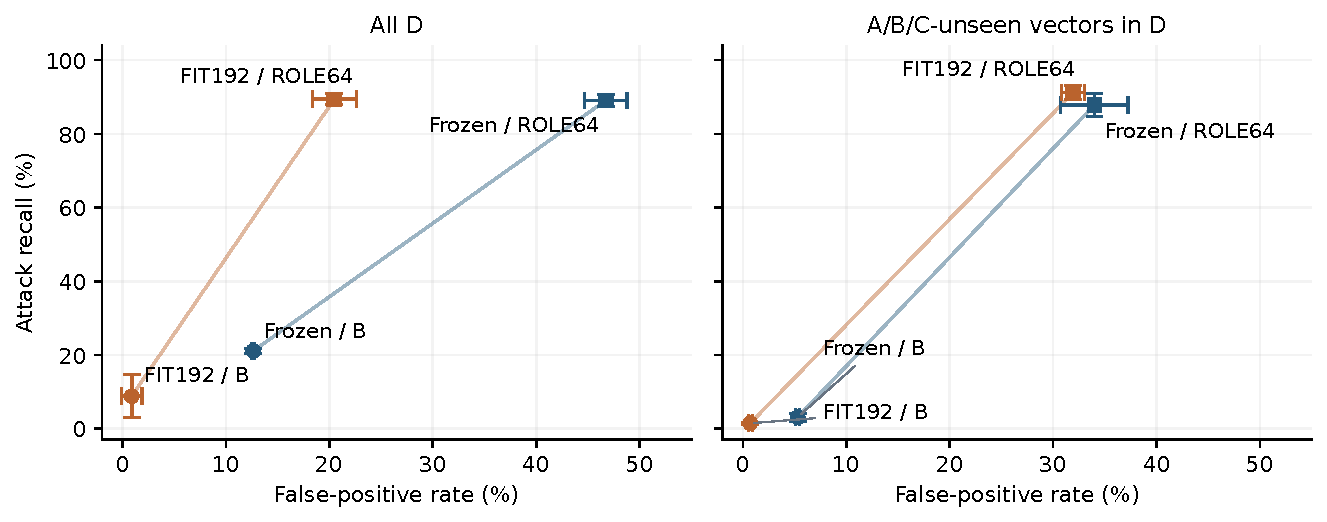
\includegraphics[width=\linewidth]{figures/fig2_operating_points.pdf}
\caption{Operating points on the same final replay. Points are seed means; bars show sample SD. Lines connect traces with identical score functions and different threshold policies, not a continuously optimized ROC curve. The large threshold effects coexist with a narrower primary comparison between the two ROLE64 traces.}
\label{fig:operating}
\Description{Operating points on the same final replay. Points are seed means; bars show sample SD. Lines connect traces with identical score functions and different threshold policies, not a continuously optimized ROC curve. The large threshold effects coexist with a narrower primary comparison between the two ROLE64 traces.}
\end{figure}

\subsection{Primary paired comparison and the joint-error criterion}
The primary contrast compares FIT192 / ROLE64 with Frozen / ROLE64. On all D, mean balanced accuracy improves by $13.28\pm2.26$ percentage points and mean block AUROC by $0.0823\pm0.0155$. Mean FP decreases by $81{,}355.4\pm6{,}051.6$. Mean FN decreases by $9{,}255.2\pm97{,}413.0$, corresponding to a recall difference of $0.29\pm3.01$ percentage points. Hence the average balanced-accuracy gain is predominantly associated with lower false-positive rates, while the missed-attack outcome is variable.

The per-seed counts in Table~\ref{tab:paired} and Figure~\ref{fig:paired} show the limitation directly. All five seeds reduce FP on the full stream, but seeds 42 and 44 increase FN. Seeds 43, 45, and 46 improve both counts. The pre-specified four-of-five criterion is therefore not met. The sign of the mean FN change does not overturn that result, and the sample SD should not be read as a confidence bound supporting superiority.

\begin{table}[tb]
\centering\small
\caption{Primary paired differences, FIT192 / ROLE64 minus Frozen / ROLE64. Negative values indicate fewer errors. Seeds 43, 45, and 46 jointly improve FN and FP in both reporting scopes; seed 44 worsens both on A/B/C-unseen vectors.}
\label{tab:paired}
\begin{tabular}{crrrr}
\toprule
 & \multicolumn{2}{c}{All D} & \multicolumn{2}{c}{A/B/C-unseen vectors} \\
\cmidrule(lr){2-3}\cmidrule(lr){4-5}
Seed & $\Delta$FN & $\Delta$FP & $\Delta$FN & $\Delta$FP \\
\midrule
\tablerows{tables/paired_rows.tex}
\bottomrule
\end{tabular}
\end{table}

\begin{figure}[tb]
\centering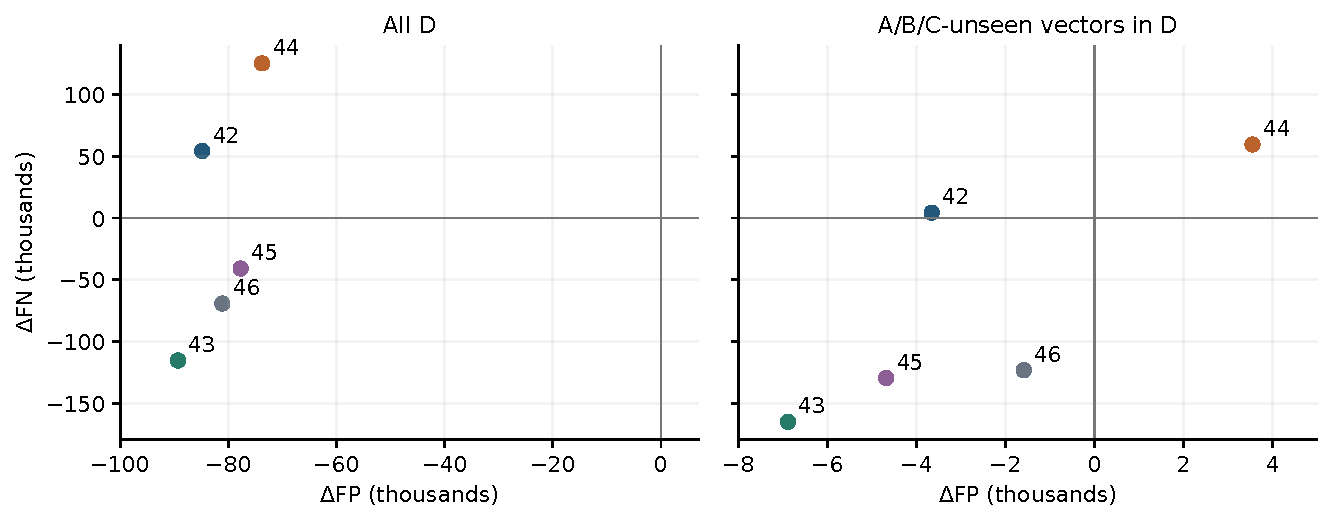
\includegraphics[width=\linewidth]{figures/fig3_paired_deltas.pdf}
\caption{Primary paired differences by seed. Both axes show thousands of errors. Joint improvement requires a point in the lower-left quadrant (including a non-deteriorating boundary). The horizontal scales differ to make the much smaller unseen-vector FP changes visible.}
\label{fig:paired}
\Description{Primary paired differences by seed. Both axes show thousands of errors. Joint improvement requires a point in the lower-left quadrant (including a non-deteriorating boundary). The horizontal scales differ to make the much smaller unseen-vector FP changes visible.}
\end{figure}

\subsection{Previously unobserved vectors and concentration of the FP gain}
For D vectors absent from A/B/C, FIT192 / ROLE64 reaches $91.20\%$ attack recall but an FPR of $31.94\%$. The corresponding Frozen / ROLE64 rates are $87.83\%$ and $33.99\%$. The paired BA gain is $2.71\pm3.63$ percentage points, substantially smaller than the full-stream gain. Mean FN decreases by $70{,}828.6\pm97{,}060.6$ and mean FP by $2{,}655.2\pm3{,}957.2$. Again, only three of five seeds jointly improve both counts.

\begin{table}[tb]
\centering\small
\caption{Complementary overlap strata in the original campaign: mean $\pm$ seed SD. Rates are percentages. The same adaptive trajectory supplies both strata.}
\label{tab:strata}
\begin{tabular}{llrrr}
\toprule
Stratum & Trace & Recall & FPR & BA \\
\midrule
\tablerows{tables/strata_rows.tex}
\bottomrule
\end{tabular}
\end{table}

The complementary seen stratum exposes the trade-off (Table~\ref{tab:strata}). Head adaptation lowers recall from 91.41\% to 86.02\%, while FPR falls from 55.96\% to 12.16\%. It adds 61,573.4 mean FN while removing 78,700.2 FP. In the unseen stratum it removes 70,828.6 FN and 2,655.2 FP. Thus the small full-stream mean FN reduction combines effects with opposite signs. The seen stratum contributes 96.7\% of the total FP reduction, but that percentage describes the location of FP savings rather than the fraction of all benefit caused by overlap. The strata differ in traffic composition and share one adaptive state.

The factorial BA interaction is positive in every original full-stream seed: 10.76--17.65 percentage points, with mean 13.55. On unseen vectors it ranges from $-4.43$ to $+4.89$ points, with mean 1.24. The gain from jointly changing the head and threshold therefore depends on the reporting population. The four-trace interaction and the complementary-stratum decomposition reveal information concealed by a single average BA gain.

\subsection{When limited labels prevent adaptation}
Label availability creates a distinct temporal failure mode in the C development replay. There are 440 skipped update decisions, all associated with insufficient recent normal examples for calibration. The longest consecutive sequence spans decision blocks 241--663 and affects predictions in blocks 242--664: 423 blocks. Figure~\ref{fig:gating} shows the eligible normal-label count and the corresponding decision rates.

\begin{figure}[tb]
\centering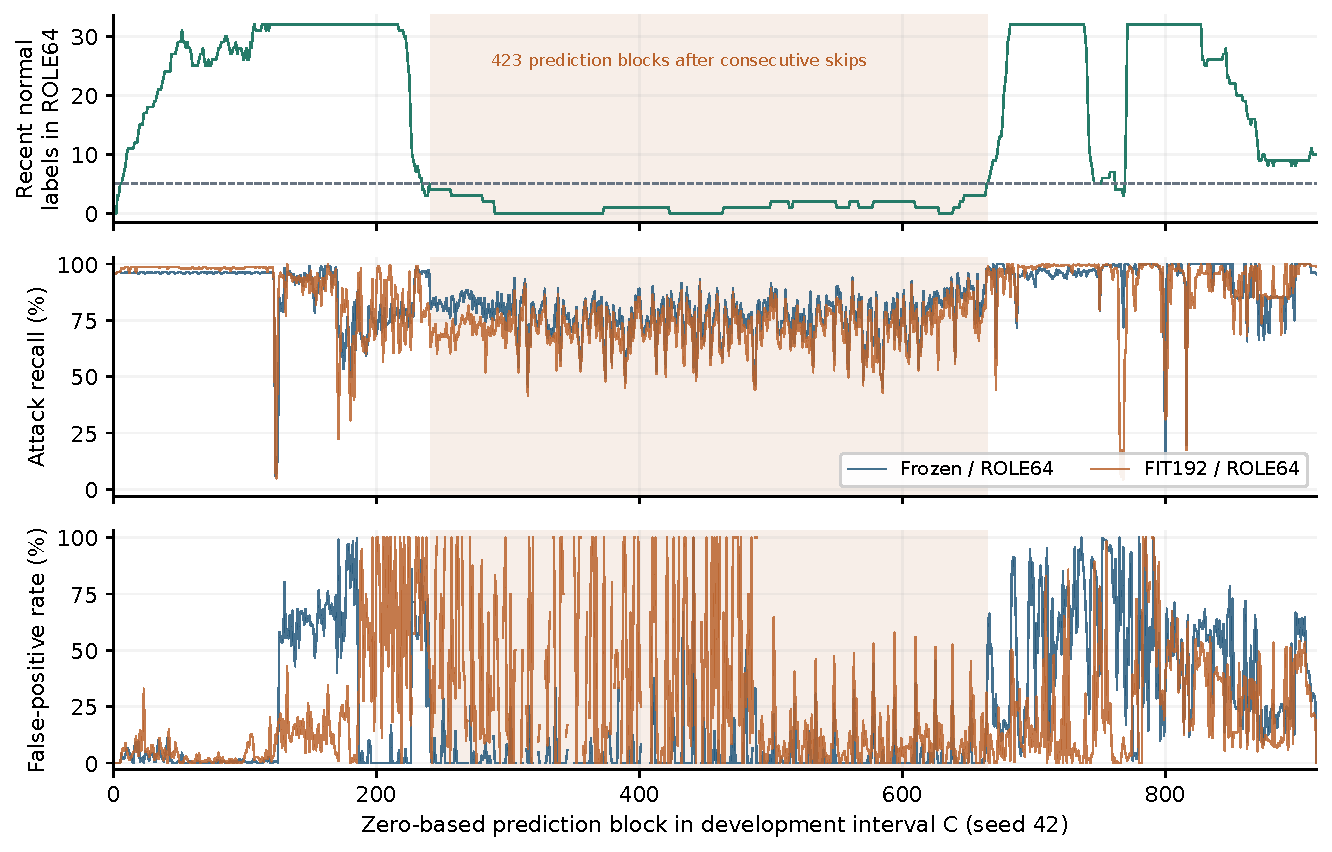
\includegraphics[width=\linewidth]{figures/fig4_development_gating.pdf}
\caption{Development interval C, seed 42. Shading marks prediction blocks 242--664, following 423 consecutive skipped update decisions. The upper panel shows the recorded number of recent normal examples in ROLE64, with the minimum of five indicated. Recall and FPR are per-block values; undefined class-specific rates remain gaps. The display is descriptive and does not randomize the occurrence of skips.}
\label{fig:gating}
\Description{Development interval C, seed 42. Shading marks prediction blocks 242--664, following 423 consecutive skipped update decisions. The upper panel shows the recorded number of recent normal examples in ROLE64, with the minimum of five indicated. Recall and FPR are per-block values; undefined class-specific rates remain gaps. The display is descriptive and does not randomize the occurrence of skips.}
\end{figure}

Stratifying predictions by the preceding update decision yields opposite FN patterns. Across 474 blocks following applied updates, FIT192 / ROLE64 has 29,697 fewer FN and 26,528 fewer FP than Frozen / ROLE64. Across 440 blocks following skips, it has 263,032 more FN and 1,342 fewer FP. In the longest skipped segment alone, both counts worsen: FN increases by 219,608 and FP by 807. These are post hoc associations conditioned on the realized stream. The segments have different class composition and cannot establish that skipping caused the deterioration.

The final D replay behaves differently. Of 354 recorded update opportunities per seed, 337, 351, 347, 341, and 350 are accepted for seeds 42--46, respectively. Their 17, 3, 7, 13, and 4 skips all occur before the first valid update. There is no recurrence of the long post-update starvation interval observed on C. The historical D record shows a different eligibility pattern from development C.

\subsection{Measured computation and its boundary}
Table~\ref{tab:cost} gives recorded computational costs on the original evaluation machine: Windows 11, Python 3.13.2, NumPy 2.3.4, scikit-learn 1.7.2, an Intel processor reported as Family 6 Model 186 Stepping 3, 12 visible CPU threads, and 16,067.4 MiB of system RAM. These are elapsed times from one execution environment, not cross-device benchmarks.

\begin{table}[tb]
\centering\small\setlength{\tabcolsep}{4.5pt}
\caption{Recorded final-run costs in seconds. Fits and threshold-selection times are components included within replay time, not extra times to add to it. The final recorded update has no subsequent evaluated block.}
\label{tab:cost}
\begin{tabular}{crrrrrr}
\toprule
Seed & Updates & Skips & Head fit & Frozen threshold & Adapted threshold & D replay \\
\midrule
\tablerows{tables/cost_rows.tex}
\bottomrule
\end{tabular}
\end{table}

The five-seed command takes 1,234.388 seconds within its recorded timer boundary. This includes D hashing and loading, initial A fitting and B preparation, the five D replays, and writing the five per-seed reports. It excludes the earlier A/B/C hash calculation and final summary serialization. Within each replay, accumulated head-fitting time is 9.630--10.672 seconds; each of the two accumulated threshold-selection components is below 0.11 seconds. These observations support only the relative cost of these implementation components in this run. They do not establish an energy advantage, a device-level latency guarantee, or an embedded memory footprint.
\FloatBarrier

